\documentclass{beamer}
\usepackage[french]{babel}
\usepackage[utf8]{inputenc}
\usepackage[T1]{fontenc}
\usepackage{subfigure}
\usepackage{listings}
\usepackage{hyperref}
\usepackage[labelformat=empty]{caption}
\usepackage{ulem}
\usetheme{Boadilla}
% \usetheme{Pittsburgh}
\definecolor{mygreen}{rgb}{0,0.6,0}
\definecolor{mygray}{rgb}{0.5,0.5,0.5}
\definecolor{mymauve}{rgb}{0.58,0,0.82}
\newcommand{\A}{\mathcal{A}}
\newcommand{\B}{\mathcal{B}}
\renewcommand{\v}{\textbf{v}}
\newcommand{\x}{\textbf{x}}
\newcommand{\p}{\textbf{p}}
\newcommand{\pA}{\ensuremath{{\bf p_\mathcal{A}}}}
\newcommand{\pB}{\ensuremath{{\bf p_\mathcal{B}}}}
\newcommand{\pone}{\ensuremath{{\bf p_1}}}
\newcommand{\ptwo}{\ensuremath{{\bf p_2}}}
\newcommand{\pii}{\ensuremath{{\bf p_i}}}
\newcommand{\pj}{\ensuremath{{\bf p_j}}}
\newcommand{\n}{\ensuremath{{\bf n}}}
\renewcommand{\a}{\ensuremath{{\bf a}}}
\DeclareMathOperator*{\argmax}{arg\,max}
\graphicspath{{src/figs/}}
\date{13 décembre 2013}

\usepackage{algorithm2e}
\usepackage{algorithmic}

\hypersetup{
    bookmarks=true,         % show bookmarks bar?
    unicode=false,          % non-Latin characters in Acrobat’s bookmarks
    pdftoolbar=true,        % show Acrobat’s toolbar?
    pdfmenubar=true,        % show Acrobat’s menu?
    pdffitwindow=false,     % window fit to page when opened
    pdfstartview={FitH},    % fits the width of the page to the window
    pdftitle={My title},    % title
    pdfauthor={Author},     % author
    pdfsubject={Subject},   % subject of the document
    pdfcreator={Creator},   % creator of the document
    pdfproducer={Producer}, % producer of the document
    pdfkeywords={keyword1} {key2} {key3}, % list of keywords
    pdfnewwindow=true,      % links in new window
    colorlinks=true,        % false: boxed links; true: colored links
    linkcolor=magenta,          % color of internal links (change box color with linkbordercolor)
    citecolor=green,        % color of links to bibliography
    filecolor=magenta,      % color of file links
    urlcolor=cyan           % color of external links
}

\lstset{ %
  backgroundcolor=\color{white},   % choose the background color; you must add \usepackage{color} or \usepackage{xcolor}
  basicstyle=\footnotesize,        % the size of the fonts that are used for the code
  breakatwhitespace=false,         % sets if automatic breaks should only happen at whitespace
  breaklines=true,                 % sets automatic line breaking
  captionpos=b,                    % sets the caption-position to bottom
  commentstyle=\color{mygreen},    % comment style
  deletekeywords={...},            % if you want to delete keywords from the given language
  escapeinside={\%*}{*)},          % if you want to add LaTeX within your code
  escapechar=−,
  extendedchars=true,              % lets you use non-ASCII characters; for 8-bits encodings only, does not work with UTF-8
  frame=single,                    % adds a frame around the code
  keepspaces=true,                 % keeps spaces in text, useful for keeping indentation of code (possibly needs columns=flexible)
  keywordstyle=\color{black},       % keyword style
  language=Ruby,                 % the language of the code
  morekeywords={*,...,f64,RigidBody,fn},            % if you want to add more keywords to the set
  numbers=none,                    % where to put the line-numbers; possible values are (none, left, right)
  numbersep=5pt,                   % how far the line-numbers are from the code
  numberstyle=\tiny\color{mygray}, % the style that is used for the line-numbers
  rulecolor=\color{black},         % if not set, the frame-color may be changed on line-breaks within not-black text (e.g. comments (green here))
  showspaces=false,                % show spaces everywhere adding particular underscores; it overrides 'showstringspaces'
  showstringspaces=false,          % underline spaces within strings only
  showtabs=false,                  % show tabs within strings adding particular underscores
  stepnumber=2,                    % the step between two line-numbers. If it's 1, each line will be numbered
  stringstyle=\color{mymauve},     % string literal style
  tabsize=2,                       % sets default tabsize to 2 spaces
  title=\lstname                   % show the filename of files included with \lstinputlisting; also try caption instead of title
}

% \lstset{emph={%  
%         let, for, \&mut%
%     },emphstyle={\color{orange}}%
% }%

\DeclareMathOperator*{\argmin}{arg\,min}
\title{Simulation temps réel d'objets rigides}
\author{Sébastien Crozet}

\begin{document}
\maketitle

\section{Pourquoi un moteur physique ?}
\begin{frame}{Motivation}
\end{frame}

\begin{frame}{Les objets rigides}
\end{frame}

\begin{frame}{Ce qui ne sera pas abordé}
    \begin{figure}[h]
        \setcounter{subfigure}{0}
        \subfigure[Joints]{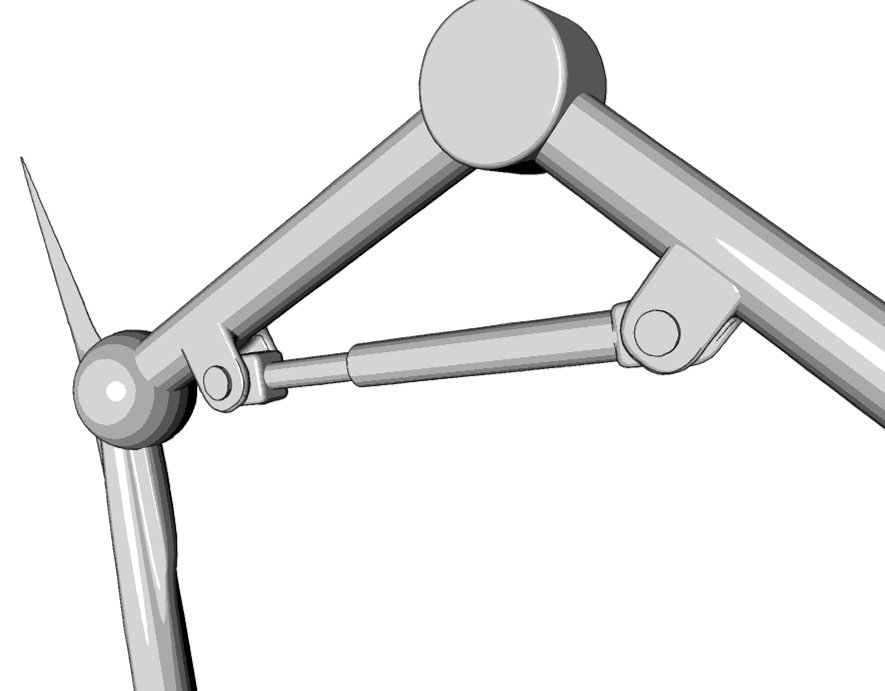
\includegraphics[height=.25\linewidth]{joint}}
        \pause
        \subfigure[Soft bodies]{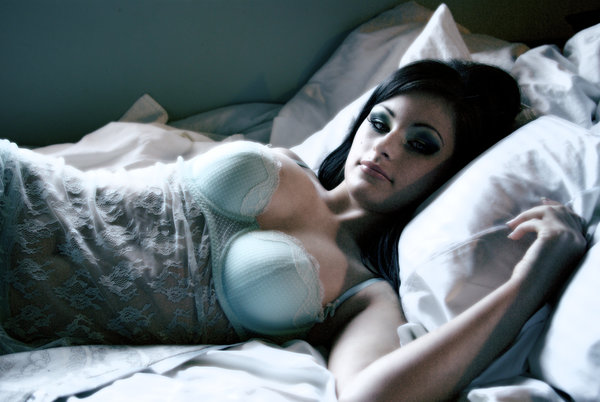
\includegraphics[height=.25\linewidth]{soft_body}}
        \pause
        \subfigure[Lancer de rayons]{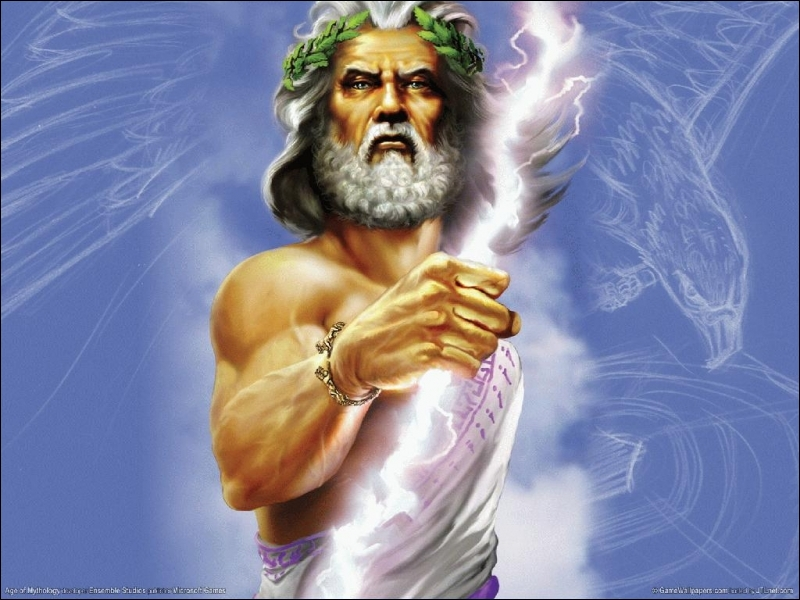
\includegraphics[height=.25\linewidth]{ray_casting}}
    \end{figure}
\end{frame}

\begin{frame}{Moteurs open-source célèbres (ou pas)}
    \begin{itemize}
        \item \textbf{2D:} Box 2d (Erin Catto)
            \begin{center}
                
\includegraphics[height=.15\linewidth]{box2d}
            \end{center}
        \item \textbf{3D:} Bullet physics (Erwin Courmand)
            \href{http://www.bulletphysics.org/Bullet/phpBB3/}{www.bulletphysics.org}
            \begin{center}
                
\includegraphics[height=.15\linewidth]{bullet_physics}
            \end{center}
            \pause
        \item \textbf{2D et 3D (générique):} Pas du tout célèbre, mais existe!
    \end{itemize}
\end{frame}

\section{Architecture}
\begin{frame}[fragile]{Architecture}
\begin{lstlisting}
fn update(bodies: &mut [RigidBody], dt: f64) {
    −\color{red}{integrate}−(bodies, dt);
    let collisions = −\color{red}{detect\_collisions}−(bodies, dt);
    let forces = −\color{red}{compute\_forces}−(bodies, collisions, dt);
    −\color{red}{apply\_forces}−(bodies, forces, dt);
}
\end{lstlisting}
\only<2>{
    \begin{figure}[h]
        \begin{center}
            
\includegraphics[scale=0.5]{rust}
            \caption{Cet exemple est écrit en Rust \href{www.rust-lang.org}{www.rust-lang.org}}
        \end{center}
    \end{figure}
}

\end{frame}

\begin{frame}[fragile]{Architecture}
\vfill
\begin{center}
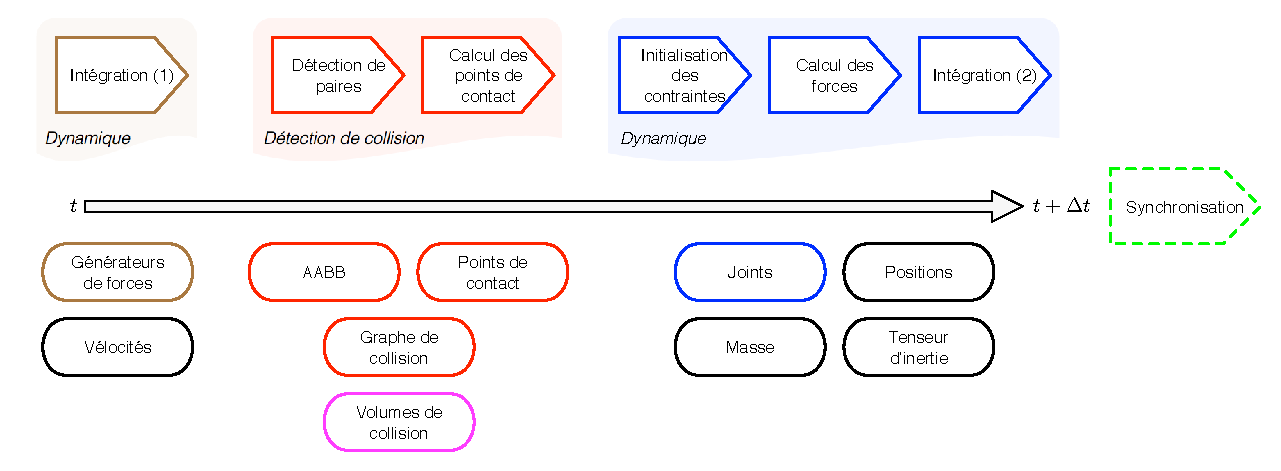
\includegraphics[scale=0.5]{workflow}
\end{center}
\vfill
\end{frame}

\section{Algorithmique de base}
\begin{frame}{L'intégration}
    \only<1>{
    \begin{block}{Problème}
        Soit $\x(t)$ la position d’un objet rigide au temps $t$, $\v(t) =
        \dot{\x}(t)$ sa vélocité, et $\a$ son accélération constante.\\
        Trouver la position et la vélocité de l’objet au temps $t + \Delta t$.
    \end{block}
    }
    \only<2->{
    \begin{itemize}
        \item Euler explicite (instable):
            \[
                \left\{
                \begin{array}{ccl}
                    \v(t + \Delta t) & = & \v(t) + \Delta t * \a\\
                    \x(t + \Delta t) & = & \x(t) + \Delta t * \v(t)\\
                \end{array}
                \right.
            \]
            \pause
        \item Euler semi-implicite (stable):
            \[
                \left\{
                \begin{array}{ccl}
                    \v(t + \Delta t) & = & \v(t) + \Delta t * \a\\
                    \x(t + \Delta t) & = & \x(t) + \Delta t * \v(t \textcolor{red}{+ \Delta t})
                    \only<3> {
                        \\
                        \boldsymbol\omega(t + \Delta t) & = & \boldsymbol\omega(t) + \Delta t * \boldsymbol\alpha\\
                        \boldsymbol\theta(t + \Delta t) & = & \boldsymbol\theta(t) + \Delta t * \boldsymbol\omega(t \textcolor{red}{+ \Delta t})\\
                    }
                \end{array}
                \right.
            \]
    \end{itemize}
    }
\end{frame}

\begin{frame}{La détection de collision}
    \only<1> {
    \begin{block}{Problème}
        Soient $n$ objets rigides. Trouver les points et normales de contact
        entre les objets qui se touchent.
    \end{block}
    }
    \only<2> {
    \begin{figure}[h]
        \setcounter{subfigure}{0}
        \subfigure[Entrée]{
\includegraphics[height=.25\linewidth]{contact_nocontact}}
        \subfigure[Sortie]{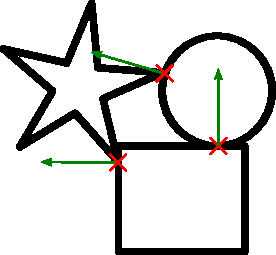
\includegraphics[height=.25\linewidth]{contact}}
    \end{figure}
    \pause
    \textbf{Il y a $n * (n - 1) / 2$ paires à tester en tout !}
    }
\end{frame}

\begin{frame}{La détection de collision}
    Que fait-on de ça ?
    \begin{center}
        
\includegraphics[scale=0.75]{penetration}
    \end{center}
    \pause
    \begin{itemize}
        \item On dit que les objets sont en \textbf{pénétration}.
            \pause
        \item La \textbf{pénétration}, c’est pas beau, et n’arrive jamais dans
            la vie réelle.
            \pause
        \item On mesure la \textbf{profondeur de pénétration}.
    \end{itemize}
    \begin{center}
        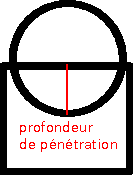
\includegraphics[scale=0.75]{penetration_depth}
    \end{center}
\end{frame}

\begin{frame}{Algorithme: boule vs. boule}
    \only<1> {
        \begin{block}{Problème}
            Soient $\A$ et $\B \subset \mathbb{R}^n$ deux boules.
            On note $r_\A$ et $r_\B \in \mathbb{R}$ leurs rayon, $\pA$et $\pB \in
            \mathbb{R}^n$ leurs position.  Calculer l’éventuelle collision.
        \end{block}
    }
    \only<2-> {
    \only<2> {
        \framesubtitle{Cas de la séparation}
        \begin{figure}[h]
            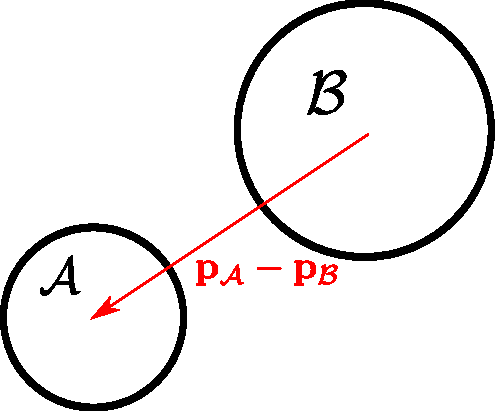
\includegraphics[height=.25\linewidth]{balls_nocollide}
        \end{figure}
        \begin{itemize}
            \item $|| \pA - \pB || > r_\A + r_\B \Rightarrow $ pas de collision.
        \end{itemize}
    }
    \only<3> {
        \framesubtitle{Cas du contact}
        \begin{figure}[h]
            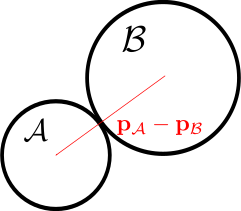
\includegraphics[height=.25\linewidth]{balls_touching}
        \end{figure}
        \begin{itemize}
            \item $|| \pA - \pB || = r_\A + r_\B \Rightarrow $ collision.
            \item normale de contact: $\n = \frac{\pA - \pB}{|| \pA - \pB ||}$.
            \item point de contact: $\pB + \n * r_\B$.
        \end{itemize}
    }
    \only<4> {
        \framesubtitle{Cas de la pénétration}
        \begin{figure}[h]
            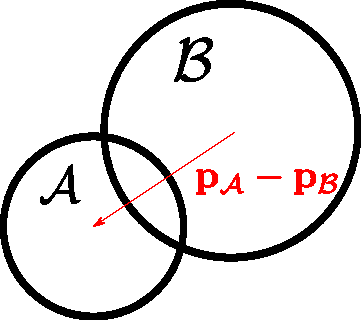
\includegraphics[height=.25\linewidth]{ball}
        \end{figure}
        \begin{itemize}
            \item $|| \pA - \pB || < r_\A + r_\B \Rightarrow $ pénétration.\\
            \item Profondeur de pénétration: $r_\A + r_\B - || \pA - \pB ||$.
        \end{itemize}
    }
    }

\end{frame}

\begin{frame}[fragile]{Algorithme: objet convexe vs. plan}
    \only<1> {
    \begin{block}{Problème}
        Soit $\A$ une partie convexe de $\mathbb{R}^n$, et
        $\mathcal{P}$ un plan (demi-espace) de normale $\n$ et de position $\p$.
        Calculer l’éventuelle collision.
    \end{block}
    }
    \only<2-> {
        \only<2> {
            \framesubtitle{Notion de convexité}
                \mbox{}\\
                $\A$~convexe~$\Leftrightarrow \forall \pone, \ptwo \in \A^2, \forall \lambda \in [0, 1], \lambda *
                \pone + (1 - \lambda) * \ptwo \in \A$
                \begin{figure}[h]
                    \setcounter{subfigure}{0}
                    \subfigure[Convexe]{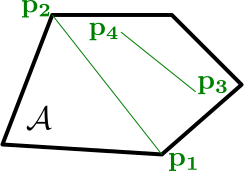
\includegraphics[height=.25\linewidth]{convexe}}
                    \subfigure[Concave]{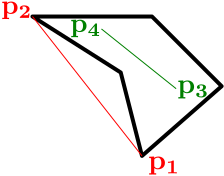
\includegraphics[height=.25\linewidth]{concave}}
                \end{figure}
        }
       \only<3> {
            \framesubtitle{Cas de la séparation}
           \begin{center}
               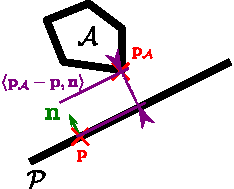
\includegraphics[height=.25\linewidth]{convex_vs_plan_nocolide}
           \end{center}
           \begin{itemize}
               \item $\left< \pA - \p, \n \right> > 0 \Rightarrow$ pas de collision.
               \item on ne sais pas (pour le moment) trouver $\pA$\ldots
           \end{itemize}
       }
       \only<4> {
            \framesubtitle{Cas du contact}
           \begin{center}
               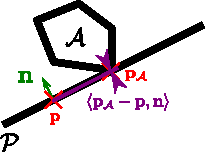
\includegraphics[height=.25\linewidth]{convex_vs_plan_contact}
           \end{center}
           \begin{itemize}
               \item $\left< \pA - \p, \n \right> = 0 \Rightarrow$ pénétration.
               \item normale de contact: $\n$.
               \item point de contact: $\pA$.
           \end{itemize}
       }
       \only<5> {
            \framesubtitle{Cas de la pénétration}
           \begin{center}
               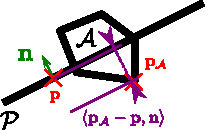
\includegraphics[height=.25\linewidth]{convex_vs_plan_penetration}
           \end{center}
           \begin{itemize}
               \item $\left< \pA - \p, \n \right> < 0 \Rightarrow$ pénétration.
               \item Profondeur de pénétration: $\left< \pA - \p, \n\right>$.
           \end{itemize}
       }
   %\begin{description}
       %\item
        \only<6,7> {
            \framesubtitle{Déterminer $\pA = s_\A(-\n)$}
        %\item[Fonction de support:]\mbox{}\\
                \begin{itemize}
                    \item On définit la \textbf{fonction de support} $s_\A(\v)$
                        de $\A$:
                        \[
                            s_\A(\v) = \argmax\limits_{\p \in \A} \left< \p, \v \right>
                        \]
                \end{itemize}
                \visible<7> {
                    \begin{center}
                        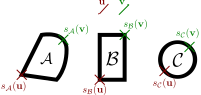
\includegraphics[height=.25\linewidth]{support_fun}
                    \end{center}
                }
        }
        \only<8> {
            \framesubtitle{Algorithme final}
            \begin{algorithm}[H]
            \begin{algorithmic}[1]
                \STATE $\pA  = s_\A(-\n)$
                \STATE $d = \left< \pA - \p, \n \right>$
                \IF{$d > 0$}
                    \RETURN Pas de collision.
                \ENDIF
                \RETURN (normale: $\n$, point: $\pA - \n * d$, pénétration: $d$)
            \end{algorithmic}
            \end{algorithm}
                \begin{center}
                    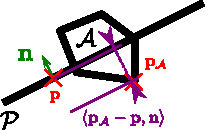
\includegraphics[height=.15\linewidth]{convex_vs_plan_penetration}
                \end{center}
        }
    }
    %\end{description}
\end{frame}

\begin{frame}{Théorie: objet convexe vs. objet convexe}
    \only<1> {
    \begin{block}{Problème}
        Soient $\A$ et $\B$ deux parties convexes de
        $\mathbb{R}^n$, trouver $\pii \in \A$ et $\pj \in
        \B$, tels que $|| \pii - \pj || = 0$.
    \end{block}
    }
    \only<2-> {
        \framesubtitle{La somme de Minkowski}
    \only<2-4> {
    \begin{itemize}
        \item<2-4> Soit $\A \oplus -\B = \{ \pii + (-\pj) \mid \pii \in
            \A \text{ et } \pj \in \B \}$\\
            Deux objets sont en collision ssi $0_{\mathbb{R}^n} \in
            \A \oplus -\B$.
        \item<3-4> Les points les plus proches entre $\A$ et
            $\B$ sont donnés par: \[ \argmin\limits_{\pii \in
            \A, \pj \in \B} || \pii - \pj || \]
        \item<4> La plus petite distance est donnée par:
            \[ \min\limits_{\pii \in \A,
            \pj \in \B} || \pii - \pj || \]
            C’est la distance entre $\A \oplus -\B$ et l’origine~!
    \end{itemize}
    }
    \only<5> {
        \begin{center}
            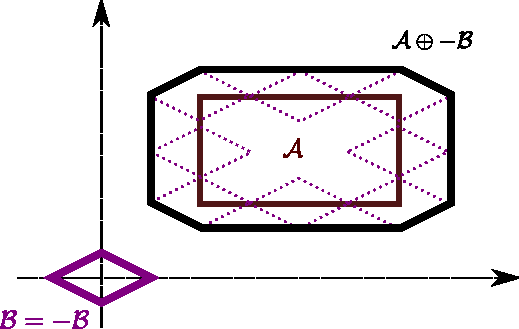
\includegraphics[scale=0.9]{a_plus_minus_b}
        \end{center}
    }
    \only<6> {
        \begin{center}
            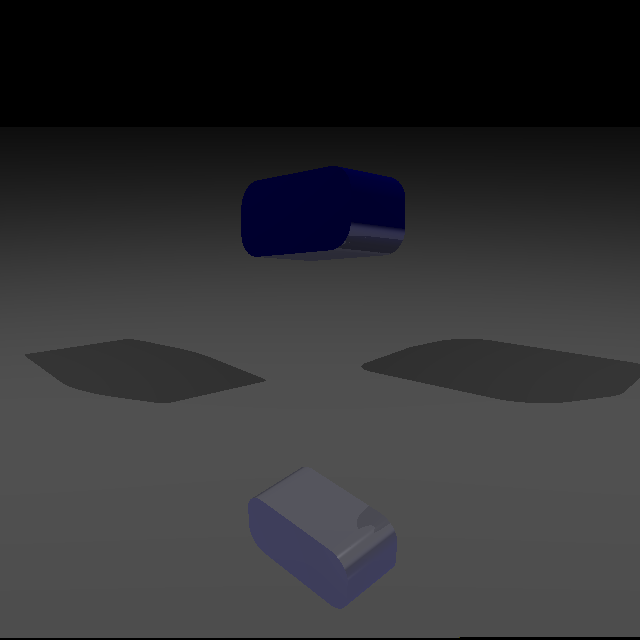
\includegraphics[scale=0.25]{box_plus_cylinder}\\
            Boite $\oplus$ 
        \end{center}
    }
    \only<7-> {
    \begin{itemize}
        \item<7-> $\A \oplus \B$ est la \textbf{Somme de Minkowski} de $\A$ et $\B$.
        \item<8-> $\A \oplus - \B$ est le \textbf{Configuration Space Obstacle} (CSO).
        \item<9-> Le CSO est très lourd à calculer explicitement.
        \item<10-> Mais sa fonction de support est facile à évaluer:
            \[
                s_{\A \oplus - \B}(\v) = s_\A(\v) - s_\B(\v)
            \]
    \end{itemize}
    }
    }
\end{frame}

\begin{frame}{Algorithme: objet convexe vs. objet convexe}
\end{frame}

\begin{frame}{Impliquant des objets concaves}
    \begin{enumerate}
        \item Décomposer en parties convexes (une fois pour toutes).
        \item Calculer les collisions entre parties convexes.
    \end{enumerate}
    \begin{center}
        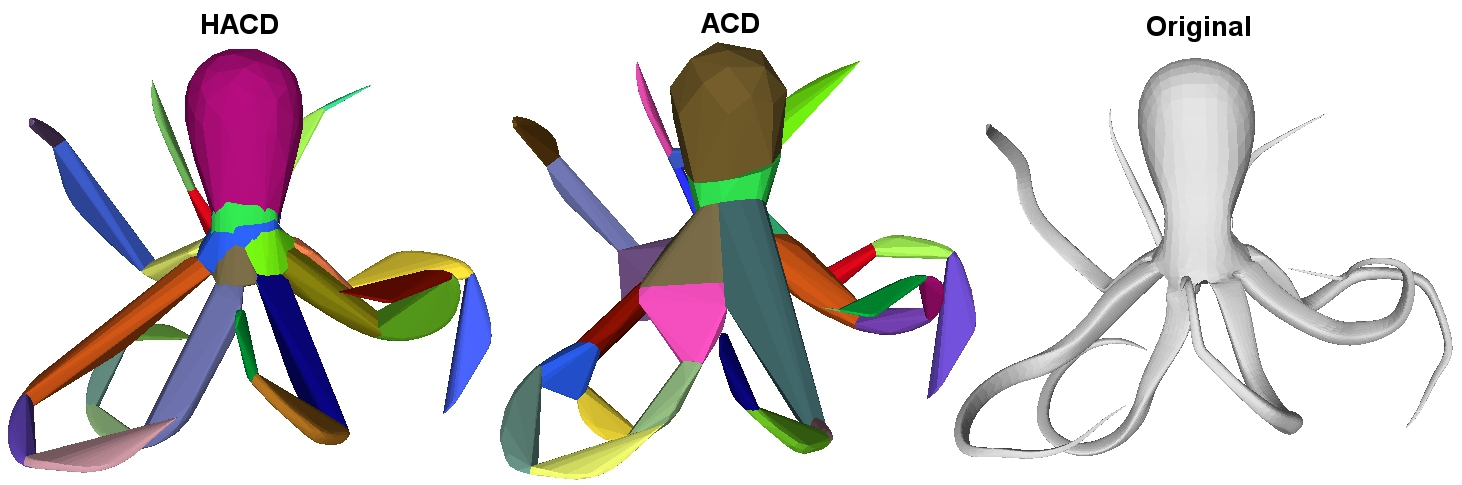
\includegraphics[height=.25\linewidth]{decomp_3d}\\
        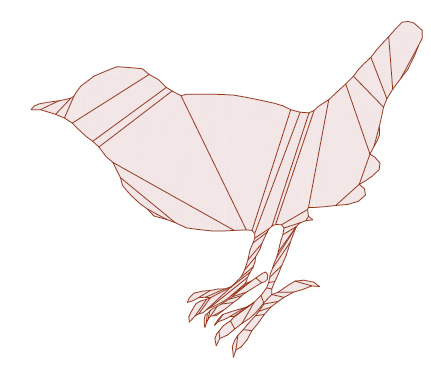
\includegraphics[height=.25\linewidth]{decomp_2d}
    \end{center}
\end{frame}

\begin{frame}{Le calcul des forces}
    \begin{block}{Problème}
         Soit un ensemble de $n$ contacts $c_i, i \in [1, n]$. Quels sont les
         forces à appliquer aux objets afin qu’ils réagissent de manière
         réaliste?
    \end{block}
    \pause
    Il suffit de résoudre le (M)LCP:
    \[
    \left\{
        \begin{array}{l}
            JM^{-1}J^T {\color{red}{\lambda}} = \zeta +
            J^T(V^1 - M^{-1}F * \Delta t)\\
            \lambda^- \leq {\color{red}{\lambda}} \leq \lambda^+ % +\infty
        \end{array}
    \right.
    \]
    \begin{center}
        
\includegraphics[height=.25\linewidth]{scared_cat}
    \end{center}
\end{frame}

\section{Amélioration des performances}
\begin{frame}{Génération de surface de contacts}
    \begin{itemize}
        \item Les algorithmes présentés ne calculent qu’un seul point de contact.
        \item C’est rarement suffisant et provoque des vibrations:
    \end{itemize}
    \begin{center}
        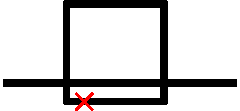
\includegraphics[scale=0.5]{acc_contact_1}
        \pause
        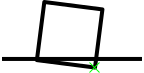
\includegraphics[scale=0.5]{contact_2}
        \pause
        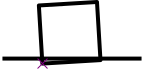
\includegraphics[scale=0.5]{contact_3}
        \pause
        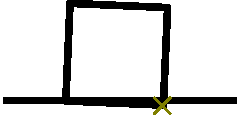
\includegraphics[scale=0.5]{contact_4}
        \pause
        
\includegraphics[scale=0.5]{contact_5}
        \pause
    \end{center}

    \textbf{Solution:} accumuler les contacts sur plusieurs frames en maximisant la
    dispersion des points.
    \pause
    \begin{center}
        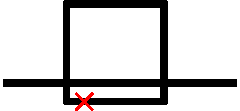
\includegraphics[scale=0.5]{acc_contact_1}
        \pause
        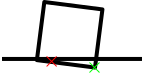
\includegraphics[scale=0.5]{acc_contact_2}
        \pause
        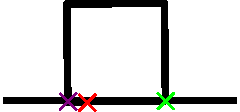
\includegraphics[scale=0.5]{acc_contact_3}
        \pause
        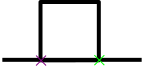
\includegraphics[scale=0.5]{acc_contact_4}
    \end{center}
\end{frame}

\begin{frame}{La Broad Phase}
    \begin{itemize}
        \item Tester les $n * (n - 1) / 2$ paires de collisions est
            impraticable!
        \item Il faut tester les collisions de manière approximative avant de
            faire les calculs les plus lourds.
    \end{itemize}
    \pause
    \begin{description}
        \item[Volumes anglobants:]
    \end{description}
    \begin{center}
        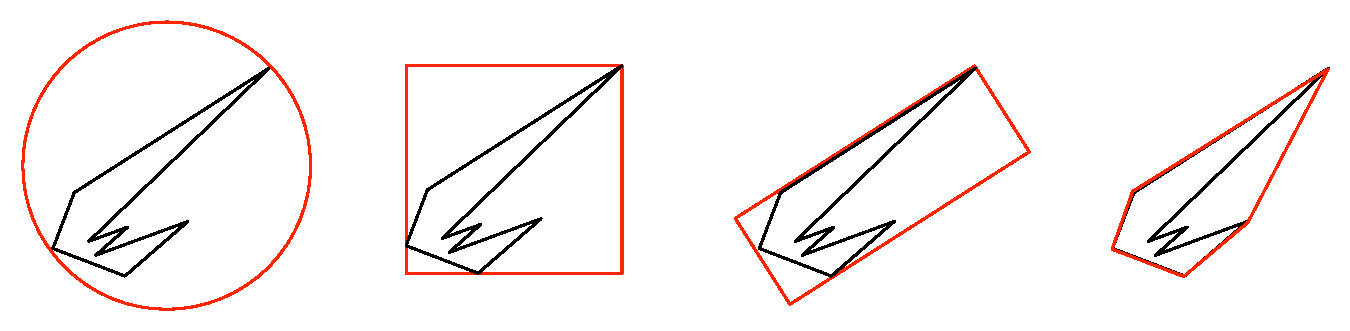
\includegraphics[scale=0.5]{bounding_volumes}
    \end{center}
\end{frame}

\begin{frame}{La Broad Phase}
    Les volumes anglobants peuvent former un arbre:
    \begin{center}
            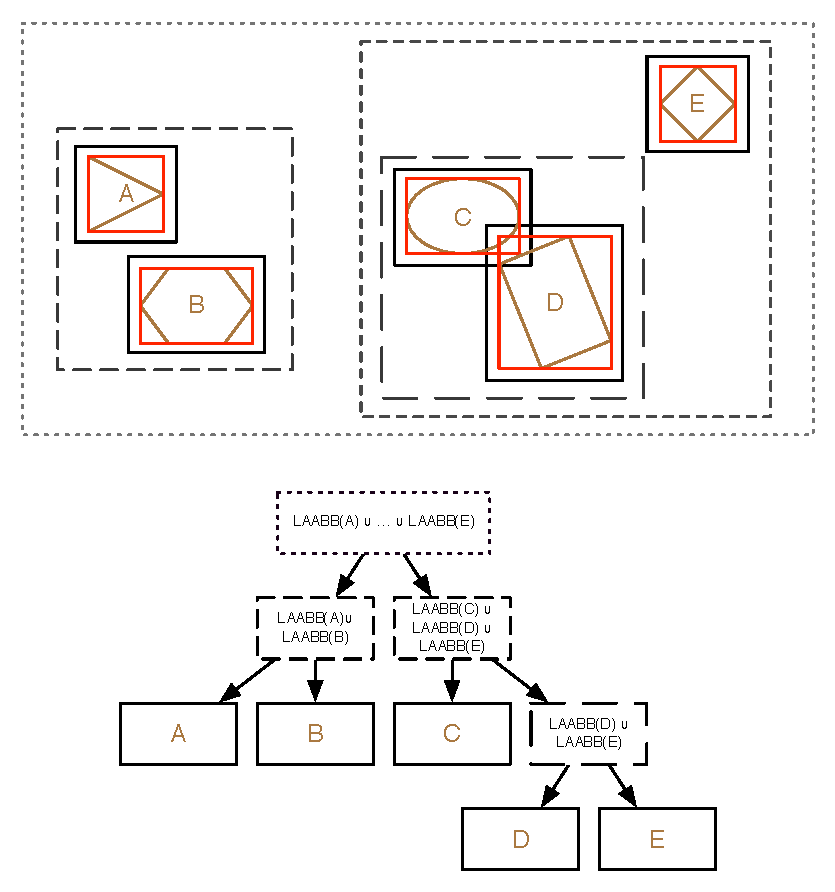
\includegraphics[scale=0.5]{AABB_tree}
    \end{center}
\end{frame}

\begin{frame}{L'endormissement}
    \begin{itemize}
        \item La plupart du temps l’utilisateur n’intéragit qu’avec
            peu d’objets. Pourquoi simuler la physique des objets immobiles?
        \pause
        \item Il faut détecter les groupes d’objets immobiles et les
            ignorer.
    \end{itemize}
        \pause
    \begin{description}
        \item[Pseudo énergie cinétique:]\mbox{}
            \[
                E(t) = m * \v^2 + \boldsymbol\omega^t * I * \boldsymbol\omega
            \]
        \pause
    \item[Recency Weighted Average:]\mbox{}
        \[
            \begin{array}{lcl}
                E_{rwa}(0) & = & E_{\text{max}}\\
                E_{rwa}(t + \Delta t) & = & \alpha * E_{rwa}(t) + (1 - \alpha) * E(t + \Delta t)\\
                E_{rwa}(t + \Delta t) & = & \min(E_{rwa}(t + \Delta t), E_{\text{max}})\\
            \end{array}
        \]
    \end{description}
    \pause
    Si $E_{rwa}$ est trop bas pour un groupe d’objets en contact, ils peuvent
    être désactivés (aka. endormis).
\end{frame}

\section{Références}
\end{document}
